\chapter{Programación Dinámica}

\section{Introducción}

La programación dinámica es una técnica de programación que se utiliza para resolver problemas computacionales. Se basa en la idea de descomponer un problema en subproblemas más pequeños y resolverlos de manera recursiva. Luego, se almacenan los resultados de los subproblemas para evitar tener que volver a calcularlos en el futuro. De esta forma, se reduce la complejidad del problema original y se obtiene una solución más eficiente.

Podríamos decir que la programación dinámica es una generalización de la técnica de divide y vencerás, ya que también se basa en la idea de descomponer un problema en subproblemas más pequeños. Sin embargo, a diferencia de divide y vencerás, la programación dinámica se utiliza cuando los subproblemas se solapan, es decir, comparten soluciones parciales. En estos casos, la programación dinámica es más eficiente, ya que evita tener que resolver los mismos subproblemas varias veces. Cuando trabajamos con soluciones con backtracking, cabe destacar que la programación dinámica viene a ser una mejora de esta técnica, ya que evita tener que recalcular los mismos subproblemas.

\section{Problema de la mochila para explicar la programación dinámica}
¿Qué objetos deberías robar para obtener el mayor valor posible en dinero?

\begin{figure}[h]
    \centering
    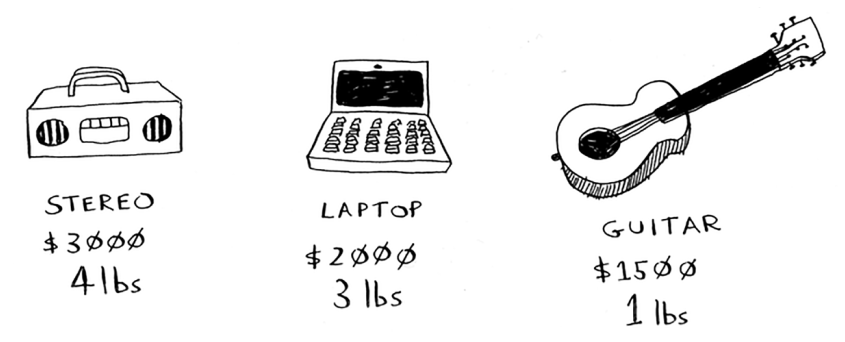
\includegraphics[width=0.7\textwidth]{estáticos/figura11.png}
    \caption{Problema de la mochila}
\end{figure}

El algoritmo más simple es este: probas con cada conjunto posible de objetos y encuentras el conjunto que te da el mayor valor.

\begin{figure}[h]
    \centering
    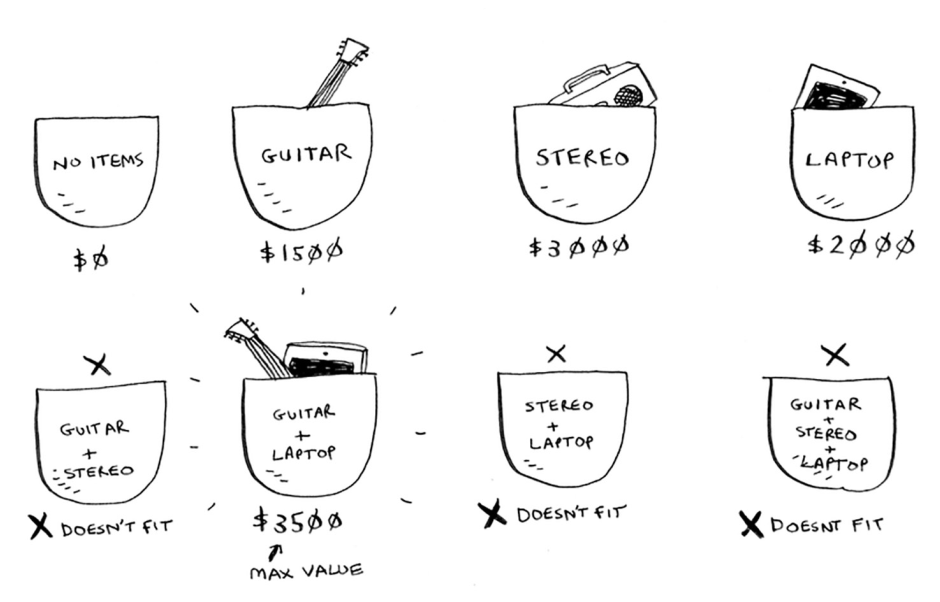
\includegraphics[width=0.6\textwidth]{estáticos/figura12.png}
    \caption{Algoritmo de fuerza bruta para el problema de la mochila}
\end{figure}

Esto funciona, pero es realmente lento. Para 3 objetos, hay que calcular 8 conjuntos posibles. Para 4 objetos, calcular 16 conjuntos. Con cada objeto que agregas el número de conjuntos que tienes que calcular se duplica. Este algoritmo toma un tiempo de O($2^n$), lo cual es muy, muy lento y es el visto anteriormente como \textit{backtracking}.

\newpage
\textbf{¿Cómo podemos hacerlo más rápido?} Con \textit{programación dinámica}, comienza resolviendo subproblemas y se va construyendo hasta resolver el problema principal. Para el problema de la mochila, comienza resolviendo el problema para mochilas más pequeñas (o “sub-mochilas”) y luego trabajar hasta resolver el problema original.

\begin{figure}[h]
    \centering
    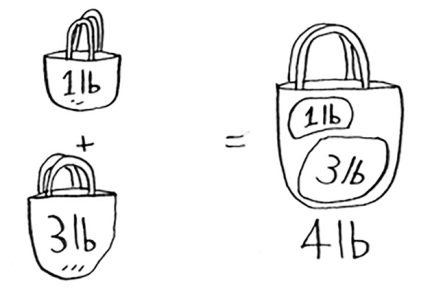
\includegraphics[width=0.4\textwidth]{estáticos/figura13.png}
    \caption{Algoritmo de programación dinámica para el problema de la mochila}
\end{figure}

¿En que se basa la programación dinámica que lo hace más rápido? En lugar de calcular el valor de cada conjunto posible de objetos, se calcula el valor de cada objeto en cada capacidad de mochila posible. Luego, se usa esa información para calcular el valor de los objetos en una mochila de mayor capacidad. De esta forma, se evita tener que recalcular los mismos subproblemas una y otra vez. Todo problema de programación dinámica comienza con una tabla, en este caso puede ser de esta forma:

\newpage
\begin{figure}[h]
    \centering
    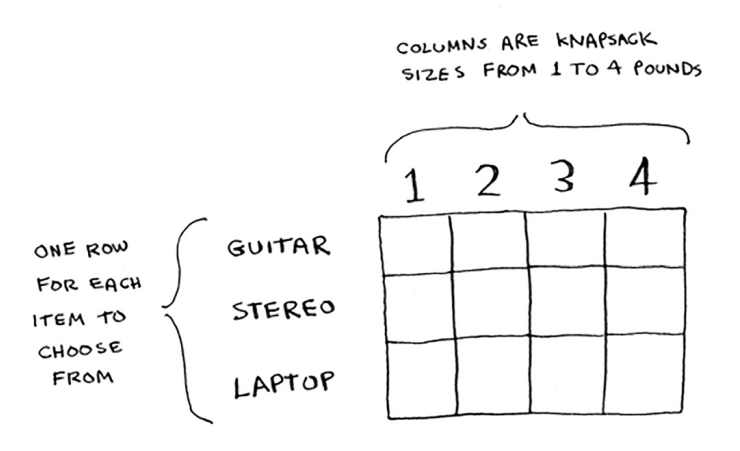
\includegraphics[width=0.65\textwidth]{estáticos/figura14.png}
    \caption{Tabla de programación dinámica para el problema de la mochila}
\end{figure}

Las filas de la cuadrícula son los objetos, y las columnas son los pesos de la mochila desde 1 lb hasta 4 lb. Necesitas todas esas columnas porque te ayudarán a calcular los valores de las sub-mochilas. La cuadrícula comienza vacía. Se va a llenar cada celda de la cuadrícula. Una vez que la cuadrícula esté llena, se tiene la respuesta al problema final.

Cuando te posiciones la fila de la guitarra, lo que significa que estás tratando de meter la guitarra en la mochila. En cada celda, hay una decisión simple: ¿Colocas la guitarra o no? Recuerda, estás tratando de encontrar el conjunto de objetos a robar que te dará el mayor valor.
La primera celda tiene una mochila con una capacidad de 1 lb. La guitarra también pesa 1 lb, ¡lo que significa que cabe en la mochila! Entonces, el valor de esta celda es \$1,500, y contiene una guitarra. Así se llenaria la tabla completa de esta forma:

\begin{figure}[h]
    \centering
    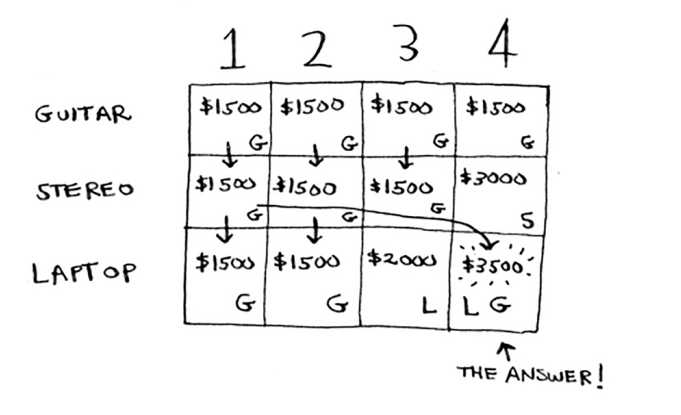
\includegraphics[width=0.45\textwidth]{estáticos/figura15.png}
    \caption{Tabla de programación dinámica para el problema de la mochila}
\end{figure}

Para calcular las demas celdas, el criterio es el siguiente: si el objeto cabe en la mochila, se calcula el valor de la mochila sin el objeto y se le suma el valor del objeto. Si el objeto no cabe en la mochila, se copia el valor de la celda de arriba. De esta forma, se va llenando la tabla hasta que se llega a la celda de la esquina inferior derecha, que contiene el valor de la mochila con todos los objetos.


\newpage
\section{Programación dinámica formalmente en el lenguaje de la materia}
Veamos por ejemplo el problema de la moneda:

\begin{codebox}{Problema del cambio de monedas con programación dinámica}
\begin{pascallike}
fun cambio(d:array[1..n] of nat, k: nat) ret r: nat
    var cam: array[0..n,0..k] of nat
    for i:= 0 to n do cam[i,0]:= 0 od
    for j:= 1 to k do cam[0,j]:= $\infty$ od
    for i:= 1 to n do
        for j:= 1 to k do
            if d[i] > j then cam[i,j]:= cam[i-1,j]
            else cam[i,j]:= min(cam[i-1,j],1+cam[i,j-d[i]])
            fi
        od
    od
    r:= cam[n,k]
end fun
\end{pascallike}
\end{codebox}

Así podemos ver la tabla de la solución del problema de las monedas:

\begin{figure}[h]
    \centering
    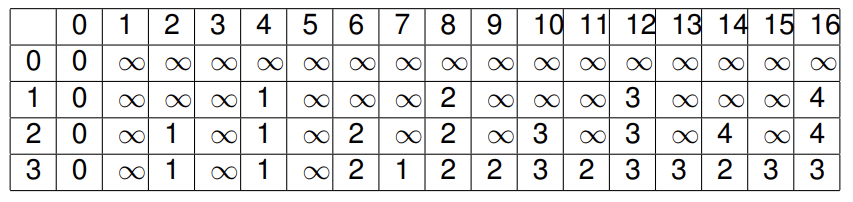
\includegraphics[width=0.8\textwidth]{estáticos/figura10.png}
    \caption{Tabla de programación dinámica para el problema del cambio de monedas}
\end{figure}

\subsection{Observaciones}

Siempre los problemas tienen la siguiente estructura:
\begin{itemize}
    \item Casos base: son los casos más simples y fáciles de resolver.
    \item Subproblemas: son los problemas más pequeños en los que se descompone el problema original.
    \item Soluciones parciales: son los resultados de los subproblemas.
    \item Solución final: es la solución al problema original, que se obtiene a partir de las soluciones parciales. Suele ser una llamada principal dependiendo de cuales son los parámetros de entrada.
\end{itemize}
Otras observaciones:
\begin{enumerate}
    \item Puedes usar programación dinámica cuando el problema se puede dividir en subproblemas discretos.
    \item Cada solución de programación dinámica implica una cuadrícula.
    \item Los valores en las celdas son generalmente lo que estás tratando de optimizar.
    \item Cada celda es un subproblema, así que piensa en cómo puedes dividir tu problema en subproblemas.
    \item No hay una fórmula única para calcular una solución de programación dinámica.
\end{enumerate}
